\documentclass[11pt]{article}
\usepackage[margin=1in]{geometry}
\usepackage{amsmath,amssymb}
\usepackage{booktabs}
\usepackage{graphicx}
\usepackage{subcaption}
\usepackage[hidelinks]{hyperref}
\usepackage{xcolor}
\usepackage{enumitem}
\setlist{nosep,leftmargin=1.4em}
\graphicspath{{figures/}}

\title{\vspace{-1.5em}Hierarchical Bayesian Model for Projecting\\ MLB Exit-Velocity Ability}
\author{Maria Oros}
\date{June 20, 2026}

\newcommand{\mph}{\,mph}

\begin{document}
\maketitle
\vspace{-1.2em}

\section{Task}
The goal is to estimate each hitter's \emph{underlying} average exit velocity (EV)
against MLB-level competition and project it into the 2024 season for all 647
batters in \texttt{exit\_velo\_validate\_data.csv}. The deliverable is a per-batter
2024 MLB projection with a measure of uncertainty, plus the methodology behind it.

\section{Data preparation}
The training data contain \textbf{1{,}344{,}651} batted-ball events (BBE) over
2019--2023 across three levels (MLB, AAA, AA). Preparation steps:
\begin{itemize}
  \item Normalize level labels to \{MLB, AAA, AA\}; drop the 97{,}979 rows with
        missing \texttt{exit\_velo}.
  \item Aggregate to \textbf{(batter, season, level) cells}, recording the mean EV,
        the batted-ball count $n$, and the standard error $\mathrm{se}=s/\sqrt{n}$.
        This reduces $\sim$1.3M rows to $\sim$6k cells while \emph{retaining the
        per-cell precision}, which is the quantity that should drive shrinkage.
\end{itemize}
Two features of the data dominate the modeling choice:
\begin{enumerate}
  \item \textbf{Sparsity.} Of 3{,}715 batters, 1{,}642 have a single season and
        per-season sample sizes range from 1 to $\sim$700 BBE
        (median 151, 10th percentile 4). A 4-BBE season carries almost no signal.
  \item \textbf{Cross-level projection.} About 100 of the 647 target batters have
        \emph{only} minor-league history, so projecting their MLB ability requires
        an \emph{estimated} level adjustment, not a constant.
\end{enumerate}

\section{Exploratory findings that shaped the model}
The raw level means are close (AA 87.6, AAA 87.8, MLB 88.4\mph), but the pooled
comparison is confounded by \emph{who} plays where. The decision-relevant quantity
is the \textbf{within-batter, within-season} level contrast: for the same hitter in
the same season, EV is \emph{higher in the minors than in MLB} ---
$\mathrm{AAA}-\mathrm{MLB}=+1.75\mph$ ($n=1{,}798$ pairs) and
$\mathrm{AA}-\mathrm{MLB}=+1.75\mph$. The raw \emph{cross-season} contrast flips
sign because of selection and development confounding. This motivates a model that
identifies the level effect strictly \emph{within} batter-season (Section~\ref{sec:ident}).

\section{Modeling methodology}
\subsection{Why a hierarchical (partial-pooling) model}
With most batters observed only briefly, fully separate per-batter models overfit,
while a single pooled estimate ignores real talent differences. A hierarchical model
\emph{shrinks} each batter toward the population by an amount that depends on the
precision of their data --- regression to the mean falls out automatically, and
sparse minor-league-only batters borrow strength from the league.

\subsection{Cell-level measurement-error likelihood}
Let cell $c$ belong to batter $b(c)$, season $t(c)$, level $\ell(c)$, with observed
mean $\bar y_c$ and known standard error $\mathrm{se}_c$. We model
\begin{equation}
\bar y_c \sim \mathcal{N}\!\left(\mu_c,\ \mathrm{se}_c\right),
\qquad
\mu_c = \mu_0 + \theta_{b(c)} + \eta_{b(c),t(c)} + \alpha_{\ell(c)}
        + \beta_1 a_c + \beta_2 a_c^2,
\end{equation}
where $a_c$ is age centered at the league mean (26.9). Treating $\mathrm{se}_c$ as
known measurement error is exactly what makes large-sample cells count more than
small ones.

\paragraph{Terms.}
\begin{itemize}
  \item $\theta_b$ --- latent batter ability, the object of interest. Non-centered
        parameterization $\theta_b=\sigma_\theta z_b,\ z_b\sim\mathcal N(0,1)$.
  \item $\alpha_\ell$ --- level equivalency, with \textbf{MLB as the reference}
        ($\alpha_{\text{MLB}}\equiv 0$); $\alpha_{\text{AAA}},\alpha_{\text{AA}}$ free.
  \item $\beta_1,\beta_2$ --- population age curve.
  \item $\eta_{b,t}$ --- a batter-season ``form'' intercept,
        $\eta_{b,t}=\sigma_s z_{b,t}$ (see below).
\end{itemize}

\subsection{Identification of the level effect}\label{sec:ident}
The batter-season intercept $\eta_{b,t}$ is shared across a player's cells in the
\emph{same} season. Consequently $\alpha_\ell$ is identified only by cells that share
a batter \emph{and} a season but differ in level --- precisely the clean contrast from
Section~3. Without $\eta_{b,t}$, $\alpha_\ell$ absorbs cross-season development and
selection effects and even flips sign. This single structural choice is what makes
the estimated equivalencies trustworthy.

\subsection{Priors and inference}
Weakly informative priors: $\mu_0\sim\mathcal N(89,5)$,
$\alpha\sim\mathcal N(-1.5,4)$ (wide; data-driven),
$\beta_1\sim\mathcal N(0,0.5)$, $\beta_2\sim\mathcal N(0,0.1)$,
$\sigma_\theta\sim\text{HalfNormal}(5)$, $\sigma_s\sim\text{HalfNormal}(2)$.
Inference uses NUTS (PyMC), 4 chains $\times$ 1{,}500 draws (2{,}000 tuning).
Sampling completes in $\sim$90\,s with \textbf{0 divergences} and
$\hat R\le 1.006$ for all reported parameters.

\subsection{Projecting 2024}
A batter's 2024 MLB \emph{ability} sets the level term to the MLB reference and the
form term to its mean (0):
\begin{equation}
\hat y_{b,2024} = \mu_0 + \theta_b + \beta_1 a_{b,2024} + \beta_2 a_{b,2024}^2,
\end{equation}
with a 95\% credible interval taken from the posterior. The six batters with no
history pool to the population ($\theta\sim\mathcal N(0,\sigma_\theta)$), yielding
appropriately wide intervals.

\section{Results}
\subsection{Parameter estimates}
\begin{table}[h]
\centering
\small
\begin{tabular}{lrrl}
\toprule
Parameter & Mean & 94\% HDI & Interpretation \\
\midrule
$\alpha_{\text{AAA}}$ & $+1.26$ & $[1.17,\,1.36]$ & AAA EV exceeds MLB; subtract to project up \\
$\alpha_{\text{AA}}$  & $+1.44$ & $[1.31,\,1.57]$ & AA EV exceeds MLB \\
$\beta_1$ (age)       & $-0.075$ & $[-0.103,\,-0.048]$ & gentle decline past the peak \\
$\beta_2$ (age$^2$)   & $-0.016$ & $[-0.021,\,-0.012]$ & concave; peak in mid-20s \\
$\sigma_\theta$       & $3.83$  & $[3.71,\,3.96]$ & between-batter talent SD \\
$\sigma_s$            & $1.15$  & $[1.10,\,1.20]$ & season-to-season ``form'' SD \\
\bottomrule
\end{tabular}
\caption{Posterior summaries. The estimated level equivalencies are \emph{positive}:
a minor-league hitter's EV must be adjusted \emph{downward} by $\sim$1.3--1.4\mph{}
to project MLB ability --- the opposite sign to the constant
($\text{AAA}=-2.5,\ \text{AA}=-4.5$) hard-coded in the ARIMA baseline.}
\end{table}

\subsection{2024 projections}
Projections for all 647 batters span 78.5--94.8\mph{} (mean 87.6). Uncertainty
behaves correctly: the mean 95\% interval is \textbf{3.3\mph{}} for batters with
history versus \textbf{15.0\mph{}} for cold-start batters (Figure~\ref{fig:unc}).

\subsection{2023 holdout backtest}
We refit on $\text{season}\le 2022$ and predict the observed 2023 MLB mean for the
490 batters with $\ge 50$ MLB BBE in 2023 (a stable target) and prior history. All
methods are scored on the same batter set.

\begin{table}[h]
\centering
\small
\begin{tabular}{lcccc}
\toprule
Method & RMSE & MAE & Bias & Corr \\
\midrule
\textbf{Hierarchical (this model)} & \textbf{1.96} & \textbf{1.48} & $-0.11$ & \textbf{0.73} \\
Career MLB mean (naive)            & 2.41 & 1.69 & $+0.08$ & 0.64 \\
Last MLB season (naive)            & 2.58 & 1.82 & $-0.19$ & 0.62 \\
Global mean                        & 2.85 & 2.20 & $+0.28$ & 0.00 \\
Per-batter ARIMA                   & 3.18 & 2.06 & $+0.42$ & 0.53 \\
\bottomrule
\end{tabular}
\caption{2023 holdout accuracy (mph). The hierarchical model cuts RMSE $\sim$19\%
below the best naive baseline; per-batter ARIMA is the \emph{worst} method,
beaten even by a constant --- on 3--4 noisy annual points it extrapolates spurious
trends.}
\end{table}

\begin{figure}[h]
\centering
\begin{subfigure}{0.49\textwidth}\centering
  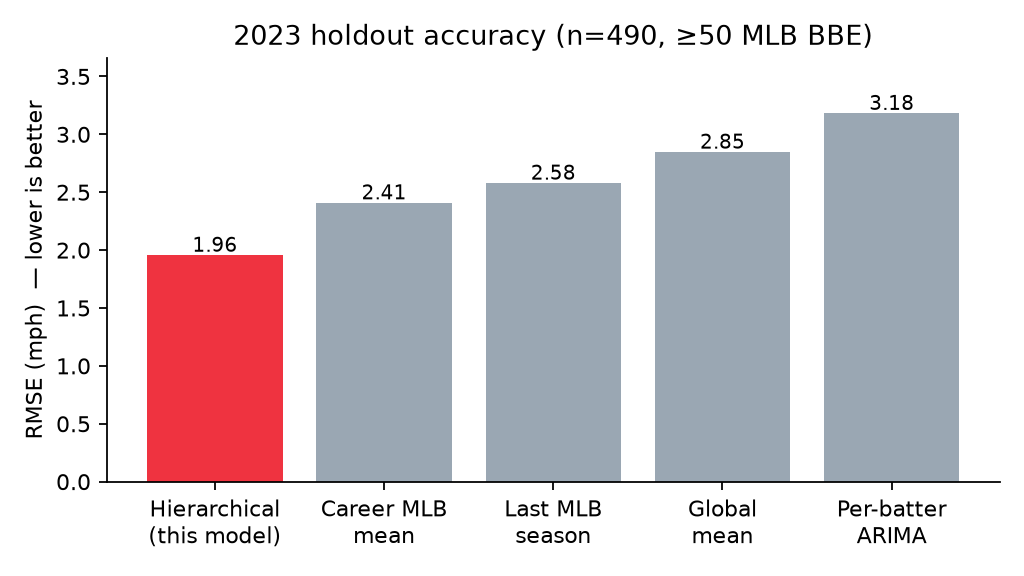
\includegraphics[width=\linewidth]{backtest_rmse.png}
  \caption{Holdout RMSE by method.}
\end{subfigure}\hfill
\begin{subfigure}{0.43\textwidth}\centering
  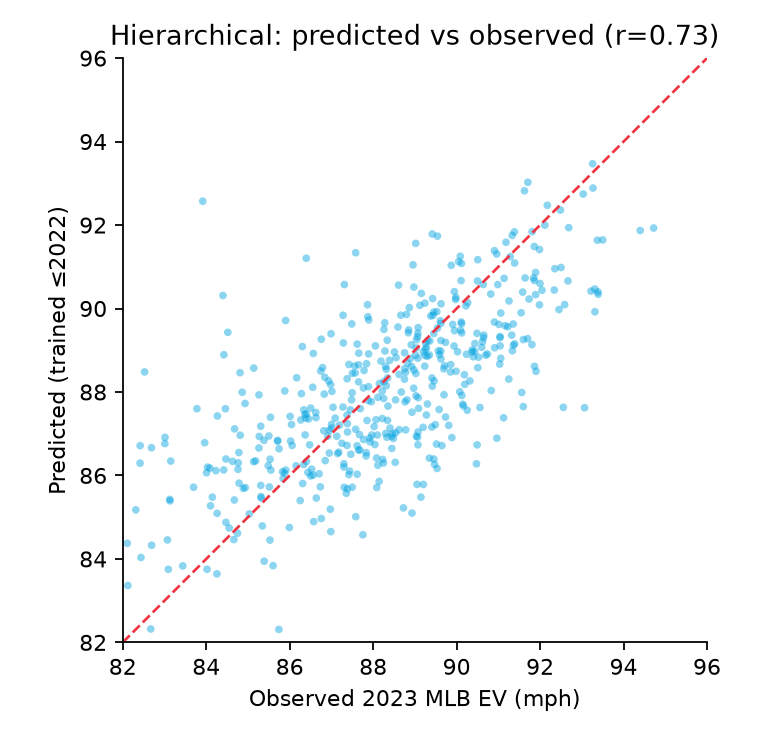
\includegraphics[width=\linewidth]{pred_vs_obs.png}
  \caption{Predicted vs.\ observed 2023.}
\end{subfigure}
\caption{The model trained only on 2019--2022 tracks held-out 2023 MLB exit velocity.}
\end{figure}

\begin{figure}[h]
\centering
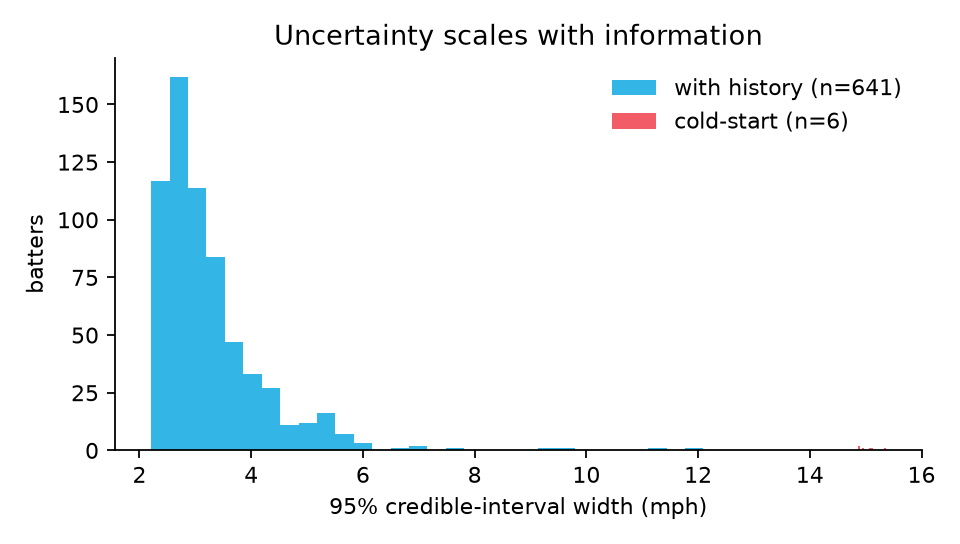
\includegraphics[width=0.62\textwidth]{uncertainty.png}
\caption{Credible-interval width by information available. Batters with playing
history get tight intervals; cold-start batters are correctly flagged as uncertain.}
\label{fig:unc}
\end{figure}

\section{Strengths, limitations, and future work}
\textbf{Strengths.} Principled sample-size shrinkage; data-estimated level
equivalencies with intervals; honest, calibrated uncertainty; and demonstrated
out-of-sample accuracy against multiple baselines.

\textbf{Limitations \& future work.}
\begin{itemize}
  \item \textbf{Quality of competition.} Pitcher identity/handedness are not yet in
        the model. A batted-ball-level extension with pitcher random effects is the
        natural next step and directly targets the prompt's QoC item.
  \item \textbf{Individual aging.} Ability is season-constant plus a \emph{population}
        age curve; player-specific development paths are not modeled.
  \item \textbf{Target noise.} The backtest target is itself a finite-sample mean;
        the $\ge 50$-BBE filter mitigates but does not remove this.
\end{itemize}

\section{Reproducibility}
All code is in the repository. The primary model is
\texttt{3\_Modeling/hierarchical/hierarchical\_model.py} (produces the 2024
projections and posterior summaries); the holdout study is
\texttt{backtest\_2023.py}. Run after \texttt{pip install -r requirements.txt};
sampling uses a fixed seed.

\end{document}
